\documentclass[12pt,a4paper]{article}

% ----- Packages -----
\usepackage[margin=1in]{geometry}
\usepackage{tikz}       % for block diagram
\usepackage{hyperref}   % clickable links
\usepackage{enumitem}   % better lists
\usepackage{amsmath, amssymb}
\usetikzlibrary{shapes, arrows.meta, positioning, backgrounds}
\usepackage[utf8]{inputenc}   % Tell LaTeX the file is UTF-8
\usepackage[T1]{fontenc}      % Use modern font encoding
\usepackage{pdflscape}
\usepackage{booktabs}
\usepackage{multirow}
\usepackage{colortbl}
\usepackage{array}

% ----- Metadata -----
\title{\textbf{Replicating Virus Isolation Protocols: Investigating FBS Concentration as a Potential Confounder in Cytopathic Effect Observation}}
\author{Albert Mathews \\ Independent Researcher}
\date{\today}

\begin{document}
\maketitle

\begin{abstract}
TODO
\end{abstract}

\section{Introduction}
This dataset aims to provide researchers in biology or artificial intelligence with images of Vero cell cultures under slightly varied conditions. This allows for comparison and contrast to understand how subtle differences can affect culture outcomes, or to train AI agents for image analysis. 

\section{Data Set Description}
\subsubsection{Data Set Availability}
The data set is available at: \url{https://doi.org/10.5281/zenodo.17928456}
\subsection{Microscope Images}
Images were obtained using an EVOS FL microscope with Bright Field or Phase illumination and 10x (400 µm scale) or 20x (200 µm scale) objectives. Scope, camera, and software details:
\begin{itemize}
    \item Microscope: EVOS® FL Auto system, Life Technologies Thermo Cat no AMAFD1000
    \item Camera: Life Technologies, high-sensitivity CMOS. Invitrogen™ EVOS™ Objectives used: AMG 10x LPlan FL PH and AMG 20x LPlan FL PH
    \item Software: DIBImage version 1.0.0 (revision 462), Evos 31201
\end{itemize}

\subsubsection{File naming}

Each image file follows this naming format: PREFIX\_pathX\_passageY\_AZZ.tif
\begin{itemize}
    \item PREFIX is either 'PREP' for the Preparation Stage, or 'EXP' for the Experiment Stage.
    \item 'X' is the path number, e.g. 1,2. PREP stage is labeled as path 1.
    \item 'Y' is the passage number, e.g. 0,1,2,3,4…10, where 0 indicates thawing.
    \item 'AZZ' is an image increment identifier. 'A' represents the day number of the passage, and 'ZZ' is an increment to ensure unique filenames.
\end{itemize}
\subsection{TEM Images}
Images were obtained using the equipment listed below.
\begin{itemize}
    \item Microscope: Tecnai G2 Spirit BioTWIN
    \item Microscope software: Tecnai version 4.6.4
    \item Camera: Milexia TEM Camera AMT Nano Sprint 43
    \item Software: AMT V701 version 7.0.1.525
\end{itemize}
\subsubsection{File naming}
Each image file is named according to this format: TEM\_pathX\_YYY\_Mag\_ZZZ.tif
\begin{itemize}
    \item “X” is the path number, e.g. 1,2.
    \item “YYY” is an image increment identifier
    \item “ZZZ” is the magnification, e.g. '4800' means 4800x magnification.
\end{itemize}

\section{Methods}
\subsection{Overview}
The diagram illustrates the experimental procedure, which includes three stages, two cell culture paths, and two culture media.
\begin{center}
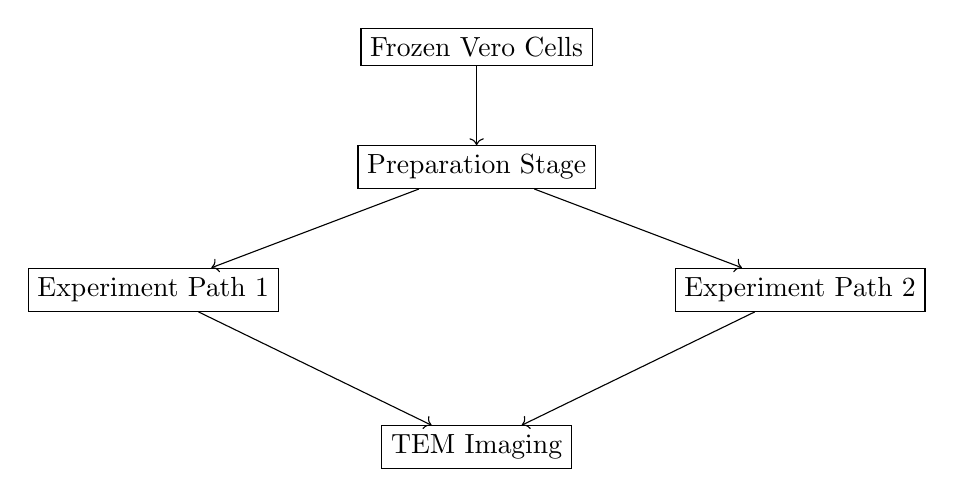
\begin{tikzpicture}[node distance=2cm, auto]
    % Example workflow
    \node (start) [draw, rectangle] {Frozen Vero Cells};
    \node (prep) [draw, rectangle, below=1cm of start] {Preparation Stage};
    \node (path1) [draw, rectangle, below left=1cm and 1cm of prep] {Experiment Path 1};
    \node (path2) [draw, rectangle, below right=1cm and 1cm of prep] {Experiment Path 2};
    \node (tem) [draw, rectangle, below=3cm of prep] {TEM Imaging};
    \draw[->] (start) -- (prep);
    \draw[->] (prep) -- (path1);
    \draw[->] (prep) -- (path2);
    \draw[->] (path1) -- (tem);
    \draw[->] (path2) -- (tem);
\end{tikzpicture}
\end{center}


\subsection{Subculturing Procedure}
The subculturing procedure followed the guidelines outlined in \cite{ATCCVERO}, specifically under 'Detailed Product Information > Handling Information > Subculturing procedure'.
\subsection{Procedure}
Describe each step in numbered order:
\begin{enumerate}[label=\arabic*.]
    \item Preparation stage: As described in [2], 'After recovery from frozen stock, Vero cells usually take 2-3 passages to reach their regular growth rate'.
    \begin{enumerate}[label=\alph*.]
        \item The thawing procedure followed \cite{ATCCVERO} > Detailed Product Information > Handling Information > Handling procedure.
        \item Cells were passaged three times during the preparation stage.
    \end{enumerate}
    \item Experiment stage: Cell cultures were split into two paths. Path 1 utilized Medium 1, and Path 2 utilized Medium 2. A single passage was conducted during the experimental stage, lasting five days.
    \item TEM stage: culture samples were prepared as follows:
    \begin{enumerate}[label=\alph*.]
    \item Sample fixing:
        \begin{enumerate}[label=\arabic*.]
            \item Discard the medium and immediately add 1.5\% or 2.5\% glutaraldehyde fixative (pH 7.0) to cover the cells.
            \item Scrape and collect the cells into a centrifuge tube.
            \item Spin down the cells, discard the supernatant.
            \item Add fixative mixed 1:1 with medium and gently pellet. 
            \item Leave at room temperature (RT) for at least 1 hr.
            \item Store at 4°C and ship with ice packs.
        \end{enumerate}
        \item Sample preparation:
        \begin{enumerate}[label=\arabic*.]
            \item Cells were fixed for at least 2 hours at RT in the above fixative. They were then washed in 0.1M cacodylate buffer and postfixed with 1\% Osmiumtetroxide (OsO4)/1.5\% Potassiumferrocyanide (KFeCN6) for 1 hour. This was followed by two washes in water, one wash in Maleate buffer (MB), and incubation in 1\% uranyl acetate in MB for 1 hour, before two final washes in water and subsequent dehydration through graded alcohol solutions (10 min each; 50\%, 70\%, 90\%, 2x10 min 100\%).
            \item Samples were then immersed in propylene oxide for 1 hour and infiltrated overnight (ON) in a 1:1 mixture of propylene oxide and TAAB Epon (TAAB Laboratories Equipment Ltd, https://taab.co.uk).
            \item The following day, samples were embedded in TAAB Epon and polymerized at 60$^{\circ}$C for 48 hours.
            \item Ultrathin sections (approximately 80 nm) were cut using a Reichert Ultracut-S microtome, collected onto copper grids, and stained with lead citrate.
        \end{enumerate}
    \end{enumerate}

\end{enumerate}

\section{Materials}
\subsection{Vero Cells}
ATCC-CRL-1586 \cite{ATCCVERO}
\subsection{Medium 1}
\begin{itemize}
    \item Eagles Minimum Essential Medium \cite{ATCCEMEM}
    \item 1x Antibiotic-Antimycotic
    \item 10\% heat-inactivated FBS
\end{itemize}
\subsection{Medium 2}
\begin{itemize}
    \item Eagles Minimum Essential Medium \cite{ATCCEMEM}
    \item 1x Antibiotic-Antimycotic
    \item 2\% heat-inactivated FBS
\end{itemize}
\subsection{Antibiotic-Antimycotic}
'1x Antibiotic-Antimycotic' refers to the following final concentrations in the growth medium:
\begin{itemize}
    \item penicillin 100 U/ml
    \item streptomycin 0.1 mg/ml
    \item amphotericin-B 0.25 $\mu$g/ml %FIXME, how to make a mu char
\end{itemize}
\subsection{Sample Fixative}
Cell samples were fixed usng the folloiwing fixtaive before being shipped to TEM lab.
2.5\% glutaraldehyde, 1.25\% paraformaldehyde, and 0.03\% picric acid in 0.1 M sodium
cacodylate buffer (pH 7.4).

\begin{thebibliography}{9}

\bibitem{ammerman2008}
Ammerman NC, Beier-Sexton M, Azad AF. Growth and maintenance of Vero cell lines. 
\textit{Current Protocols in Microbiology}. 2008 Nov; Appendix 4:Appendix 4E.  
doi:\href{https://doi.org/10.1002/9780471729259.mca04es11}{10.1002/9780471729259.mca04es11}.  
PMID: \href{https://pubmed.ncbi.nlm.nih.gov/19016439}{19016439};  
PMCID: \href{https://www.ncbi.nlm.nih.gov/pmc/articles/PMC2657228}{PMC2657228}.

\bibitem{ATCCVERO}
American Type Culture Collection, "VERO C1008 [Vero 76, clone E6, Vero E6] Product Page,"  
\url{https://www.atcc.org/products/crl-1586}, accessed July 29, 2025.

\bibitem{MilliporeSigma}
MilliporeSigma, "Vero C1008 [Vero 76, clone E6, Vero E6] Product Page,"  
\url{https://www.sigmaaldrich.com/CA/en/product/sigma/cb_85020206}, accessed July 29, 2025.

\bibitem{ATCCEMEM}
American Type Culture Collection, "Eagle's Minimum Essential Medium (EMEM) Product Page,"  
\url{https://www.atcc.org/products/30-2003}, accessed July 29, 2025.

\end{thebibliography}


\end{document}
